\section{Introduction}

%---------------------------------------------------------------------------------------------

\begin{frame}{Seems familiar?}

\begin{block}{Laws of Research Writing\ldots}
\begin{itemize}%%[noitemsep,nolistsep]
\item  Likelihood of a crash/hang is directly proportional to the importance of a document.
\item  Likelihood of a crash/hang is inversely proportional to the time left before its deadline.
\item  Likelihood of a crash/hang is directly proportional to the duration since you last saved.
\item \textit{Well, MS-Word does not crash that often now, but hangs/slows-down frequently ...}
\end{itemize}
\end{block}

\vspace{5mm}
That's enough laws for now...
\vspace{5mm}
\end{frame}

%---------------------------------------------------------------------------------------------

\begin{frame}{Requirement}
\begin{block}{Aren't you looking for something}
\begin{itemize}%%[noitemsep,nolistsep]
\item  Reliable for very reliable documents like thesis and papers.
\item  That doesn't screw-up the formatting if you press enter inadvertently.
\item  That doesn't make you re-do all the numberings, when your guide asks you put a figure somewhere in the middle.
\end{itemize}
\end{block}

\vspace{5mm}
Answer is \textcolor{green}{\LaTeX}
\end{frame}

%---------------------------------------------------------------------------------------------

\begin{frame}{\LaTeX~is\ldots}
\ldots a sophisticated document preparation system.

~\\

\begin{block}{\LaTeX~has\ldots}
\begin{itemize}
\item Stylistic uniformity
\item Bibliography support
\item Sophisticated structuring abilities
\item Reference tracking
\item Highly extendibles capabilities
\end{itemize}
\end{block}
\end{frame}

%---------------------------------------------------------------------------------------------

\begin{frame}{\LaTeX~is not\ldots}
\ldots a word processor.

~\\

\begin{block}{\LaTeX~does not\ldots}
\begin{itemize}
\item Give you complete control over formatting
\item Provide a graphical interface for editing and Spell-check your documents\footnotemark
\end{itemize}
\end{block}
``You take care of writing, and we'll take care of presentation."
\footnotetext{You can use program TeXWorks to spell check your \LaTeX \\}
\end{frame}

%---------------------------------------------------------------------------------------------
%
%\begin{frame}{A Brief History}
%It all started with Donald Knuth and \emph{The Art of Computer Programming}\ldots
%% angry about the poor typesetting quality of the second edition, he realized that printing was just 1s (ink) and 0s (no ink) and set out to make his own typesetting system.
%
%~\\
%
%\begin{itemize}
%\item \TeX~- a computer language used for typesetting math and other technical material.
%\begin{itemize}
%\item Created in the late 1970s by Donald Knuth
%\end{itemize}
%\item \LaTeX~- a higher-level method of accessing the power of \TeX
%\begin{itemize}
%\item Created in the early 1980s by Leslie Lamport
%\end{itemize}
%\end{itemize}
%
%~\\
%
%\LaTeX~is pronounced lah-tech or lay-tech.
%\end{frame}
%
%\begin{frame}{Why \LaTeX?}
%Presentation shouldn't get in the way of content.
%\begin{block}{For example\ldots}
%{\small\begin{itemize}
%\item With a word processor, you spend valuable time agonizing over what font size to make the section headings.\\
%	\hspace{.5cm}With \LaTeX, you just tell it to start a new section.
%\item With a word processor, changing the formatting means you have to change each instance individually.\\
%	\hspace{.5cm}With \LaTeX, you just redefine the relevant commands.
%\item With a word processor, you have to carefully match any provided templates.\\
%	\hspace{.5cm}With \LaTeX, you can be sure you've fit the template, and switch templates easily.
%\end{itemize}}
%\end{block}
%\end{frame}
%

%---------------------------------------------------------------------------------------------

\begin{frame}{Background}
\begin{block}{What is \LaTeX?}
\begin{itemize}%%[noitemsep,nolistsep]
\item In 1978, Donald Knuth createf a typesetting system, called Tex (pronounced 'tech') after being disappointed with the quality of his acclaimed The Art of Programming series.

\item Tex gave extremely fine-grained control of document layout. 
\item However, the vast flexibility meant it was complex, so by the mid-80s Leslie Lamport created a set of macros that abstracted away many of the complexities.
\item A simpler approach for creating documents, where content and style were separate. 
\item This extension became Latex (pronounced 'lay-tech').
\end{itemize}
\end{block}
\end{frame}

%---------------------------------------------------------------------------------------------
\begin{frame}{Background\ldots}
\begin{block}{What is \LaTeX?}
\begin{itemize}%%[noitemsep,nolistsep]
\item Latex is essentially a markup language. 
\item Content is written in plain text and can be annotated with various 'commands' 
\item The Latex interpreter reads in a Latex marked-up file, renders the content into a document and dumps it a new file. 
\item Therefore, it's not an interactive system that is the de-facto method for document creation nowadays.
\end{itemize}
\end{block}
\end{frame}

%---------------------------------------------------------------------------------------------
\begin{frame}
\frametitle{Why use \LaTeX}
   
\begin{block}{Advantages of \LaTeX}
\begin{itemize}
\item Graduate students are poor.  \LaTeX is free!
\item Available on all Windows, Mac \& Linux
\item .tex files are ASCII files and very portable are portable, and the output is in PDF, DVI or PS.
\end{itemize}
\end{block}
\end{frame}

%---------------------------------------------------------------------------------------------
\begin{frame}
\frametitle{Why use \LaTeX}
\begin{block}{Advantages of \LaTeX}
\begin{itemize}
\item Every computer can open a PDF, not so with Word or Powerpoint
\item Typesetting is much better, more professional.  This is especially true for mathematics.  Can be formatted to suit various publication styles easily.
\item Styles for different publication styles are easily available, as are Templates for letters, articles, books, reports etc. (\emph{just ask Google!})
\item Can compile huge books\ldots $\approx70,000$ pages
\item Bibliography management
\end{itemize}
\end{block}
\end{frame}

%---------------------------------------------------------------------------------------------
\begin{frame}
\frametitle{When not to use \LaTeX}
\begin{block}{Disadvantages of \LaTeX}
\begin{itemize}
\item Font selection not as easy as Word.
\item Difficult to flow text around pictures\slash figures
\item If you write few documents, or only want short documents with little math
The first time you write in \LaTeX, it will likely take longer than you would like\ldots
\item Does not \emph{directly} support drawing figures\ldots you need other software
\item Must remember commands
\item Not straightforward for creating complex tables
\end{itemize}
\end{block}
\end{frame}

%%%%%%%%%%%%%%%%%%%%%%%%%%%%%%%%
%\begin{frame}
%   \frametitle{How do I get it?}
%   \begin{itemize}
%      \item \href{http://support.math.arizona.edu/tex/}{http://support.math.arizona.edu/tex/} for all your needs
%      
%      \item Good IDEs:
%        \begin{enumerate}
%           \item Kile (\emph{Linux})
%           
%           \item TeXnicCenter (\emph{Windows})
%           
%           \item WinEdt (\emph{Windows, clearly})
%           
%           \item TeXShop (\emph{Mac})
%        \end{enumerate}
%   \end{itemize}
%\end{frame}
%

\section{Syntax}

%%-----------------------------------------------------------------------------------------
%\begin{frame}{"Hello \LaTeX!"}
%\begin{block}{Creating a \LaTeX~Document}
%\begin{itemize}
%\item Write a \texttt{.tex} file using any text editor (preferably TeXWorks)
%\end{itemize}
%{\scriptsize\hspace{2cm}\texttt{\% this is hello.tex \\
%\hspace{2cm}\textbackslash documentclass\{article\} \\
%\hspace{2cm}\textbackslash begin\{document\} \\
%\hspace{2.5cm}Hello, \textbackslash LaTeX! \\
%\hspace{2cm}\textbackslash end\{document\}}}
%\begin{itemize}
%\item Compile to produce .pdf
%\item Examples of the output, later in the presentation
%\end{itemize}
%\end{block}
%\end{frame}
%
%\subsection{Writing LaTeX Code}

%-----------------------------------------------------------------------------------------
\begin{frame}{\texttt{documentclass}}
\LaTeX~has several templates, selected using \texttt{\textbackslash documentclass}
\begin{block}{Classes:}
\begin{itemize}
\item book
\item report
\item article
\item letter
\item beamer
\end{itemize}
Etc.
\end{block}
You'll be using the `article' class for your paper
\end{frame}

%-----------------------------------------------------------------------------------------
\begin{frame}{Declarations and Environments}
\begin{block}{Declarations\ldots}
\begin{itemize}
\item Are stated once
\item Take effect until further notice
\item Can optionally be constrained
\end{itemize}
Ex. \texttt{\textbackslash documentclass}, \texttt{\textbackslash small}
\end{block}
\begin{block}{Environments\ldots}
\begin{itemize}
\item Have matching \texttt{begin} and \texttt{end} declarations
\item Must be constrained
\end{itemize}
Ex. \texttt{\textbackslash begin\{document\} \ldots \textbackslash end\{document\}}
\end{block}
\end{frame}

%-----------------------------------------------------------------------------------------
\begin{frame}{Arguments}
\begin{block}{Required arguments\ldots}
\begin{itemize}
\item Are contained in curly braces
\item Must be included
\end{itemize}
Ex. \texttt{\textbackslash documentclass\{\underline{article}\}}
\end{block}
\begin{block}{Optional arguments\ldots}
\begin{itemize}
\item Are contained in square brackets
\item Can be left out
\item Give you more control over the commands
\end{itemize}
Ex. \texttt{\textbackslash documentclass[\underline{12pt}]\{article\}}
\end{block}
\end{frame}

%-----------------------------------------------------------------------------------------
\begin{frame}{Special Characters}
\begin{itemize}
\item Another type of command
\item Don't define any formatting or structure
\item Print non-standard characters or characters which usually mean something else
\end{itemize}
Ex. \texttt{\textbackslash LaTeX}, \texttt{\textbackslash textbackslash}, \texttt{\textbackslash \%} \\
Note: \% is a reserved character because it is for comments (After a \%, the rest of the line is ignored by the compiler) \\
\end{frame}

%-----------------------------------------------------------------------------------------

\begin{frame}{Packages}
Packages allow you to further customize \LaTeX.
\begin{block}{The command:}
\hspace{1cm}\texttt{\textbackslash usepackage\{\emph{name}\}}
\end{block}
\begin{block}{Some packages:}
graphicx, epsfig, geometry, fancyhdr, setspace, amsmath, listings, xcolor, url\ldots
\end{block}
Most of the packages you'll need are already included in the template
\end{frame}

%\subsection{Basic Formatting}
%-----------------------------------------------------------------------------------------

\begin{frame}{Font Types}
\begin{block}{Font face:}
\texttt{\textbackslash emph\{}\emph{Text}\texttt{\}}, \texttt{\textbackslash textbf\{}\textbf{Text}\texttt{\}}, \texttt{\textbackslash texttt\{}\texttt{Text}\texttt{\}}, \texttt{\textbackslash textrm\{}\textrm{Text}\texttt{\}}, \texttt{\textbackslash textsf\{}\textsf{Text}\texttt{\}}, \texttt{\textbackslash textsc\{}\textsc{Text}\texttt{\}}
\end{block}
\begin{block}{Font size:}
\texttt{\{\textbackslash tiny} {\tiny Text}\texttt{\}}, \texttt{\{\textbackslash scriptsize} {\scriptsize Text}\texttt{\}}, \texttt{\{\textbackslash footnotesize} {\footnotesize Text}\texttt{\}}, \texttt{\{\textbackslash small} {\small Text}\texttt{\}}, \texttt{\{\textbackslash normalsize} {\normalsize Text}\texttt{\}}, \texttt{\{\textbackslash large} {\large Text}\texttt{\}}, \texttt{\{\textbackslash Large} {\Large Text}\texttt{\}}, \texttt{\{\textbackslash LARGE} {\LARGE Text}\texttt{\}}, \texttt{\{\textbackslash huge} {\huge Text}\texttt{\}}, \texttt{\{\textbackslash Huge} {\Huge Text}\texttt{\}}
\end{block}
%\begin{block}{Alignment:}
%\texttt{\textbackslash begin\{center/flushright/flushleft\}\\
%\ldots\\
%\textbackslash end\{center/flushright/flushleft\}}
%\end{block}
\end{frame}

%-----------------------------------------------------------------------------------------

\begin{frame}{Spacing}
\begin{block}{Margins}
{\small The default: between 1.5 inches and 1.875 inches

Setting margins: \texttt{\textbackslash usepackage[margin=\emph{0.5in}]\{geometry\}}}
\end{block}
\begin{block}{Paragraphs and other breaks}
{\small Paragraphs are separated by a blank line.

You can force a new line using \textbackslash\textbackslash

To force a new page, use \texttt{\textbackslash newpage} or \texttt{\textbackslash clearpage}}
\end{block}
%\begin{block}{Other spacing}
%{\small Force a space using $\sim$
%
%Add space using \texttt{\textbackslash hspace\{\emph{1in}\}} or \texttt{\textbackslash vspace\{\emph{1in}\}}
%
%Fill space using \texttt{\textbackslash hfill} or \texttt{\textbackslash vfill}}
%\end{block}
\end{frame}

%-----------------------------------------------------------------------------------------
\begin{frame}{Lists}
%There are two main types\ldots
\begin{block}{Bulleted lists:}
\vspace{2mm}
\begin{columns}
\column{0.6\textwidth}
\hspace{1.5cm}\texttt{\textbackslash begin\{itemize\} \\
\hspace{2cm}\text\textbackslash item} Text \\
\hspace{2cm}\texttt{\textbackslash item} Text \\
\hspace{1.5cm}\texttt{\textbackslash end\{itemize\}}
\column{0.4\textwidth}
\begin{itemize}
\item Text
\item Text
\end{itemize}
\end{columns}
\end{block}
\begin{block}{Numbered lists:}
\vspace{2mm}
\begin{columns}
\column{0.6\textwidth}
\hspace{1.5cm}\texttt{\textbackslash begin\{enumerate\} \\
\hspace{2cm}\text\textbackslash item} Text \\
\hspace{2cm}\texttt{\textbackslash item} Text \\
\hspace{1.5cm}\texttt{\textbackslash end\{enumerate\}}
\column{0.4\textwidth}
\begin{enumerate}
\item Text
\item Text
\end{enumerate}
\end{columns}
\end{block}
\end{frame}

%-----------------------------------------------------------------------------------------

%\section{\LaTeX~and You}

%\begin{frame}{Getting Started}
%Download \texttt{http://web.mit.edu/belzner/Public/latex/scigen.zip} and open \texttt{scigen.tex} in your favorite text editor

%~\\

%\hspace{1.7cm}\texttt{\% this is scigen.tex \\
%\hspace{1.7cm}\textbackslash documentclass[12pt]\{article\} \\
%\hspace{1.7cm}\textbackslash begin\{document\} \\
%\hspace{2.5cm}\ldots \\
%\hspace{1.7cm}\textbackslash end\{document\}}
%\end{frame}

%\subsection{The Files}

\begin{frame}{Typical File Structure for your Paper or Thesis}
In your \texttt{Document} can be split into several files\ldots
\begin{block}{Structure-Organization of the Document}
\begin{itemize}
\item \texttt{main.tex} brings everything together, don't edit it
%\item \texttt{preamble.tex} contains any additional packages or macros
%\item \texttt{cover.tex} contains the cover information (title, author, etc.)
\item \texttt{abstract.tex} and \texttt{summary.tex} contain the text of your scientific abstract and executive summary, respectively
\item \texttt{paper.tex} contains the main body of your paper, including any and all figures, tables, etc.
\item \texttt{biblio.bib} is a Bib\TeX~file containing your references
%\item \texttt{appa.tex} contains the text of any appendices you may have
\end{itemize}
\end{block}
Compile to generate \texttt{main.pdf}
\end{frame}

%-----------------------------------------------------------------------------------------

%\begin{frame}{The Title Page}
%\texttt{cover.tex} is where you define the content of your title page
%\begin{itemize}
%\item It includes declarations of the \texttt{title}, \texttt{author}, and \texttt{date}
%\item You should replace the title and author as needed, but leave the date alone
%\end{itemize}
%{\scriptsize\texttt{\hspace{2cm}\textbackslash title\{Length-enhanced superlative verbiage\} \\
%\hspace{2cm}\textbackslash author\{Joe Everystudent \\
%\hspace{2.5cm}\textbackslash vspace\{0.5in\}\textbackslash\textbackslash\\
%\hspace{2.5cm}under the direction of\textbackslash\textbackslash\\
%\hspace{2.5cm}Dr. Famous Person\textbackslash\textbackslash\\
%\hspace{2.5cm}Massachusetts Institute of Technology\\
%\hspace{2.5cm}\textbackslash vspace\{1in\}\}}}
%\begin{itemize}
%\item The title page is created automatically using the \texttt{maketitle} command in \texttt{main.tex}
%\end{itemize}
%\end{frame}

%-----------------------------------------------------------------------------------------
\begin{frame}{Abstract and Summary}
\begin{itemize}
\item Your final paper may have both a \textbf{technical} abstract and a \textbf{non-technical} summary
\item All you need to do is fill in the text, and the template takes care of the rest
\end{itemize}
\begin{block}{Behind the Scenes}
\hspace{1cm}\texttt{\textbackslash begin\{abstract\} \\
\hspace{1.5cm}\textbackslash input\{abstract\} \\
\hspace{1.5cm}\textbackslash vspace\{1in\} \\
\hspace{1.5cm}\textbackslash begin\{center\}\textbackslash textbf\{Summary\}\textbackslash end\{center\} \\
\hspace{1.5cm}\textbackslash input\{summary\} \\
\hspace{1cm}\textbackslash end\{abstract\}}
\end{block}
\end{frame}
%-----------------------------------------------------------------------------------------

\begin{frame}{Bibliography}
\texttt{biblio.bib} acts as a database of references, and only includes in the bibliography those references you cite in your paper
\begin{block}{Bib\TeX}
{\small\texttt{@article\{\emph{nameofentry}, \\
\hspace{0.5cm}author = \{\emph{D. Deutsch and A. Barenco and Artur Ekert}\}, \\
\hspace{0.5cm}title = \{\emph{Universality in Quantum Computation}\}, \\
\hspace{0.5cm}journal = \{\emph{Proceedings: Math and Physical Sciences}\}, \\
\hspace{0.5cm}volume = \emph{449}, \\
\hspace{0.5cm}year = \emph{1995}, \\
\hspace{0.5cm}number = \emph{1937}, \\
\hspace{0.5cm}pages = \{\emph{669--677}\} \\
\}}}
\end{block}
A more complete list of examples can be found at \url{web.mit.edu/rsi/www/pdfs/bibtex-format.pdf}
\end{frame}

%-----------------------------------------------------------------------------------------

\begin{frame}{Referencing}
\begin{block}{References}
\hspace{1cm}\texttt{\textcolor{cyan}{\textbackslash section\{Results\}}\textbackslash label\{res\} \\
\hspace{1cm}\textcolor{cyan}{\ldots\\
\hspace{1cm}As seen in Section} \textbackslash ref\{res\} \textcolor{cyan}{\ldots}}
\end{block}
\begin{block}{Footnotes}
\hspace{1cm}\texttt{\textcolor{cyan}{\ldots telephony}\textbackslash footnote\{Phony telephones\}}
\end{block}
\begin{block}{Citations}
{\small\hspace{1cm}\texttt{\textcolor{cyan}{Redundancy} \textbackslash cite\{\emph{nameofentry}\}} \\
\hspace{0.5cm}For multiple citations: \\
\hspace{1cm}\texttt{\textcolor{cyan}{\ldots methodology} \textbackslash cite\{\emph{nameofentry}, \emph{nameofotherentry}\}}}
\end{block}
\end{frame}

%-----------------------------------------------------------------------------------------
\begin{frame}{The Paper}
\LaTeX~is built off of the idea of \emph{structure} over \emph{formatting}

~\\

\hspace{1cm}\texttt{\textbackslash section\{\textcolor{cyan}{Introduction}\}}

~\\

\begin{block}{Layers of sectioning}
\hspace{2mm}{\large section}\\
\hspace{4mm}subsection\\
\hspace{6mm}{\small subsubsection}\\
\hspace{8mm}{\footnotesize paragraph}\\
\hspace{10mm}{\scriptsize subparagraph}
\end{block}
%These commands should be used as needed in both \texttt{paper.tex} and \texttt{appa.tex}
\end{frame}


%\subsection{Math Mode}
%-----------------------------------------------------------------------------------------

\begin{frame}{Typesetting Math}
\LaTeX~allows you to typeset any sort of equations.
\begin{block}{\LaTeX~math support}
$$\int_a^b\frac{d\theta}{1+\theta^2} = \tan^{-1}b - \tan^{-1}a$$
\end{block}
\begin{block}{Using math mode}
Inline math mode: \texttt{\$\ldots\$}
\begin{center}
$\int_1^\infty e^{-x} dx$~~~~$\sum_{n=0}^\infty n!$
\end{center}

Display math mode: \texttt{\$\$\ldots\$\$}

Numbered equations: \texttt{\small \textbackslash begin\{equation\}\ldots\textbackslash end\{equation\}}
\end{block}
\end{frame}

%-----------------------------------------------------------------------------------------
\begin{frame}{Some Commands}
\begin{center}
\begin{tabular}{rl}
$974$ & \texttt{\$974\$} \\
$4+2$ & \texttt{\$4+2\$} \\
$\sqrt[3]{5}$ & \texttt{\$\textbackslash sqrt[3]\{5\}\$} \\
$\frac{x}{y}$ & \texttt{\$\textbackslash frac\{x\}\{y\}\$} \\
$A^{x}_{y}$ & \texttt{\$A\^{}\{x\}\_\{y\}\$} \\
$\sum_{k=1}^n k$ & \texttt{\$\textbackslash sum\_\{k=1\}\^{}n k\$} \\
$2 \ne 4$ & \texttt{\$2 \textbackslash ne 4\$} \\
$\phi \in \Psi$ & \texttt{\$\textbackslash phi \textbackslash in \textbackslash Psi\$} \\
$\hat{\i}\times\hat{\j}=\hat{k}$ & \texttt{\$\textbackslash hat\{\textbackslash i\} \textbackslash times \textbackslash hat\{\textbackslash j\} = \textbackslash hat\{k\}\$} \\
$f''(\xi)$ & \texttt{\$f''(\textbackslash xi)\$} \\
CH$_3$COOH & \texttt{CH\$\_3\$COOH} \\
180$^{\circ}$C & \texttt{180\$\^{}\{\textbackslash circ\}\$C} \\
Coca Cola$^{\text{TM}}$ & \texttt{Coca Cola\$\^{}\{\textbackslash text\{TM\}\}\$} \\
\end{tabular}


~\\

\texttt{\textcolor{cyan}{\ldots runs in} \$\textbackslash Theta(\textbackslash log n)\$ \textcolor{cyan}{time\ldots}}
\end{center}
\end{frame}

%\subsection{Figures and Tables}

%-----------------------------------------------------------------------------------------
\begin{frame}{Figures and Tables}
Both are environments:
\begin{block}{Figures}
\hspace{1cm}\texttt{\textbackslash begin\{figure\} \\
\hspace{1.5cm}\ldots \\
\hspace{1cm}\textbackslash end\{figure\}}
\end{block}
\begin{block}{Tables}
\hspace{1cm}\texttt{\textbackslash begin\{table\} \\
\hspace{1.5cm}\ldots \\
\hspace{1cm}\textbackslash end\{table\}}
\end{block}
Positioning can be defined as an optional argument: \\
\hspace{1cm}\texttt{\textcolor{cyan}{\textbackslash begin\{figure\}}[htbp]}
\end{frame}

%-----------------------------------------------------------------------------------------
\begin{frame}{\texttt{includegraphics}}
\begin{block}{How to include pictures?}
%{\small\hspace{1cm}\texttt{\textcolor{cyan}{\textbackslash subsection\{Hardware Configuration\}} \\
%~\\
%
\hspace{1cm}\textbackslash begin\{figure\}[ht] \\
\hspace{1.5cm}\textbackslash centering \\
\hspace{1.5cm}\textbackslash includegraphics[height=3in]\{figure0.png\} \\
\hspace{1cm}\textbackslash end\{figure\} \\
~\\
\hspace{1cm}\textbackslash begin\{figure\}[ht] \\
\hspace{1.5cm}\textbackslash centering \\
\hspace{1.5cm}\textbackslash includegraphics[width=\textbackslash textwidth]\{figure1.png\} \\
\hspace{1cm}\textbackslash end\{figure\}

\end{block}
\end{frame}

%-----------------------------------------------------------------------------------------
\begin{frame}{Formatting Tables}
The \texttt{table} environment defines the figure style. The \texttt{tabular} environment defines the table itself.\\
~\\
\begin{columns}
\column{0.7\textwidth}

\textbackslash begin\{table\}[ht] \\
\hspace{.5cm}\textbackslash centering \\
\hspace{.5cm}\textbackslash begin\{tabular\}\{|r||c|c|\} \textbackslash hline \\
\hspace{1cm}Trial \& \$n\$ \& \$t\$ \textbackslash\textbackslash~\textbackslash hline \\
\hspace{1cm}1 \& 23 \& 2 \textbackslash\textbackslash~\textbackslash hline \\
\hspace{1cm}2 \& 15 \& 10 \textbackslash\textbackslash~\textbackslash hline \\
\hspace{1cm}3 \& 100 \& 20 \textbackslash\textbackslash~\textbackslash hline \\
\hspace{.5cm}\textbackslash end\{tabular\} \\
\textbackslash end\{table\}

\column{0.3\textwidth}
\begin{table}
\centering
\begin{tabular}{|r||c|c|} \hline
Trial & $n$ & $t$ \\ \hline
1 & 23 & 2 \\ \hline
2 & 15 & 10 \\ \hline
3 & 100 & 20 \\ \hline
\end{tabular}
\end{table}
\end{columns}
\end{frame}

%-----------------------------------------------------------------------------------------
\begin{frame}{Captions and Labels}
\begin{block}{Captioning}
\hspace{1cm}\texttt{\textcolor{cyan}{\textbackslash end\{tabular\}} \\
\hspace{1cm}\textbackslash caption\{The data.\}\\
\hspace{1cm}\textcolor{cyan}{\textbackslash end\{table\}}}
\end{block}
\begin{block}{Labeling}
\hspace{1cm}\texttt{\textcolor{cyan}{\textbackslash caption\{The data.\}} \\
\hspace{1cm}\textbackslash label\{\emph{nameoftable}\}\\
\hspace{1cm}\textcolor{cyan}{\textbackslash end\{table\}}}
\end{block}
\begin{block}{Referencing}
\hspace{1cm}\texttt{\textcolor{cyan}{\ldots in Table} \textbackslash ref\{\emph{nameoftable}\}}
\end{block}
\end{frame}

% %-----------------------------------------------------------------------------------------
% \section{Examples}
% {
    % \setbeamercolor{background canvas}{bg=}
    % 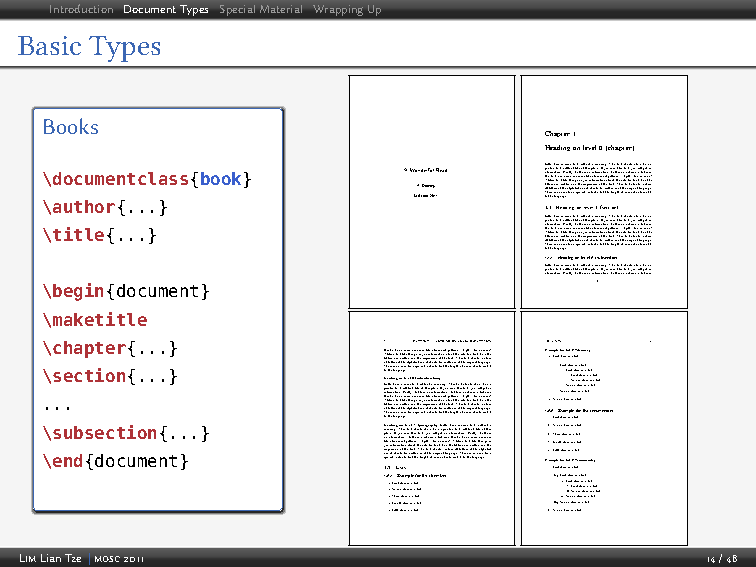
\includepdf[pages=-]{examples.pdf}
% }

%-----------------------------------------------------------------------------------------
%\section{Beamer}
%
%\begin{frame}{Getting Started}
%Beamer allows all the same commands as a normal \LaTeX~document, plus some.
%\begin{block}{Adding a Slide}
%\hspace{1cm}\texttt{\textbackslash begin\{frame\}\{\emph{Title}\} \\
%\hspace{1.5cm}\ldots \\
%\hspace{1cm}\textbackslash end\{frame\}}
%\end{block}
%\begin{block}{Special slides}
%Title slide:\\
%\hspace{1cm}\texttt{\small\textbackslash titlepage} \\
%Table of contents:\\
%\hspace{1cm}\texttt{\small\textbackslash tableofcontents[currentsection]}
%\end{block}
%\end{frame}
%
%\begin{frame}{Beamer at RSI}
%We have a template for this too! It's in the file \texttt{slides.tex}
%\begin{block}{Title Slide}
%Be sure to fill in the title, subtitle (if necessary) and author
%
%\hspace{1cm}\texttt{\textbackslash title\{Witty catch-phrase\} \\
%\hspace{1cm}\textbackslash subtitle\{Length-enhanced superlative verbiage\} \\
%\hspace{1cm}\textbackslash author[Joe Everystudent]\{Joe Everystudent\textbackslash\textbackslash \\
%\hspace{1.5cm}Research Science Institute\textbackslash\textbackslash \\
%\hspace{1.5cm}Under the Direction of Dr. Famous Person\textbackslash\textbackslash \\
%\hspace{1.5cm}Massachusetts Institute of Technology\}}
%\end{block}
%The template already includes a title slide!
%\end{frame}
%
%\begin{frame}{Formatting}
%Some special environments can be useful for presentations
%\begin{block}{Blocks}
%\hspace{1cm}\texttt{\textbackslash begin\{block\} \\
%\hspace{1.5cm}\ldots \\
%\hspace{1cm}\textbackslash end\{block\}}
%\end{block}
%\begin{block}{Columns}
%\hspace{1cm}\texttt{\textbackslash begin\{columns\} \\
%\hspace{1.5cm}\textbackslash column\{0.5\textbackslash textwidth\} \\
%\hspace{2cm}Column 1 \\
%\hspace{1.5cm}\textbackslash column\{0.5\textbackslash textwidth\} \\
%\hspace{2cm}Column 2 \\
%\hspace{1cm}\textbackslash end\{columns\}}
%\end{block}
%\end{frame}
%
%\begin{frame}{Animation}
%You can also do some basic animation in beamer.
%\pause
%\begin{itemize}
%\item \texttt{\textbackslash pause} puts a pause before revealing the rest of the slide
%\item<3-4> \texttt{\emph{command}\textless\emph{num}-\emph{num}\textgreater} makes the command apply only for some number of the ``frames''
%\item<4-> The previous bullet is defined by \texttt{\textbackslash item\textless3-4\textgreater}
%\item<5-> The bullet disappears after the fourth ``frame''
%\end{itemize}
%\end{frame}
%
%% Slide on "everything you do in normal LaTeX works in beamer too!"
%
%\begin{frame}{Themes}
%You can also choose different themes for beamer.
%\begin{block}{Design}
%\hspace{1cm}\texttt{\textbackslash usetheme\{\emph{theme}\}}
%
%Antibes, Berkeley, Berlin, Goettingen, Malmoe, Szeged, Warsaw\ldots
%\end{block}
%\begin{block}{Color}
%\hspace{1cm}\texttt{\textbackslash usecolortheme\{\emph{theme}\}}
%
%beaver, crane, lily, rose, seahorse, whale\ldots
%\end{block}
%\end{frame}
%

%\section{Common \LaTeX~Errors}
%
%%\begin{frame}{The Structure of an Error}
%%\centering
%%\includegraphics[width=\textwidth]{error.png}
%%\end{frame}
%
%\begin{frame}{Missing Closing Braces}
%\begin{block}{The Code}
%\texttt{\textbackslash includegraphics\{picture.png}
%\end{block}
%\begin{block}{The Error Message}
%\centering
%\includegraphics[width=\textwidth]{brace.png}
%\end{block}
%\end{frame}
%
%\begin{frame}{Missing Environment End}
%\begin{block}{The Code}
%\texttt{\textbackslash begin\{itemize\}\\
%\textbackslash item Text.}
%\end{block}
%\begin{block}{The Error Message}
%\centering
%\includegraphics[width=\textwidth]{end.png}
%\end{block}
%\end{frame}
%
%\begin{frame}{Spaces in Filenames}
%\begin{block}{The Code}
%\texttt{\textbackslash includegraphics\{a picture.png\}}
%\end{block}
%\begin{block}{The Error Message}
%\centering
%\includegraphics[width=\textwidth]{space.png}
%\end{block}
%\end{frame}
%
%\begin{frame}{Forgetting to Escape}
%\begin{block}{The Code}
%\texttt{a\_b}
%\end{block}
%\begin{block}{The Error Message}
%\centering
%\includegraphics[width=\textwidth]{escape.png}
%\end{block}
%\end{frame}
%
%\begin{frame}{Forgetting to Use Math Mode}
%\begin{block}{The Code}
%\texttt{\textbackslash frac\{1\}\{2\}}
%\end{block}
%\begin{block}{The Error Message}
%\centering
%\includegraphics[width=\textwidth]{math.png}
%\end{block}
%\end{frame}

\section{Conclusion}
%
%\begin{frame}{So, why \LaTeX?}
%\begin{itemize}
%\item \LaTeX~allows you to worry about the content and the structure, rather than the presentation.
%\item \LaTeX~has one of the most advanced math typesetting systems around.
%\item \LaTeX~is incredibly extendible.
%\item \LaTeX~keeps track of references so you don't have to.
%\item \LaTeX~allows you to make more consistent, and more easily changeable, documents.
%\end{itemize}
%\end{frame}

%----------------------------------------------------------------------------------------------
\begin{frame}{What is so special about \LaTeX \thickspace compared to Word?}
\begin{tabular}{@{}p{0.45\linewidth} | p{0.45\linewidth}@{}}\toprule
\textbf{\LaTeX} & \textbf{Word}\\ \midrule
Text, Open source, Free 		& Binary, Proprietary, Paid \\
Version neutral				& May not be forward-backward compatible\\
TeX is guaranteed to be bug free. The author, Stanford Professor Donald Knuth, will send you a reward check is you find a bug. The reward is currently USD 327.68 & Have you seen Word misbehave? not? lucky!!\\
TeX documents are small and lean. & What's the smallest Word file on your computer?\\
On Linux, Mac, Windows		& Native to Windows but other ports are available\\
\bottomrule
\end{tabular}
\end{frame}

%---------------------------------------------------------------------------------------------

\begin{frame}{Advantages of \LaTeX}
\begin{tabular}{@{}p{0.45\linewidth} | p{0.45\linewidth}@{}}\toprule
\textbf{\LaTeX} & \textbf{Word}\\ \midrule
Contents can be split into multiple files,  can be included in multiple documents-presentations, update syncs & No straight forward sub-file inclusion\\
Templates  auto-format. Useful for Conference and Journal papers. Switching is easy & Limited template support\\
Auto numbering, indexes, bibliography & Limited auto-index support, like ToC\\
Compiles the files, so renumbering is possible quickly & renumbering is manual and painful \\
Excellent Math formatting & Limited Math equations\\
%Using SVG for vector graphics is better, as picture is stored parametrically and does not distort on scaling & Pictures in jpg, png, gif distort on scaling as they are stored as pixel\\
Bibliography, citations are very effective using jabref & referring and formatting them is pain\\
\bottomrule
\end{tabular}
\end{frame}
%---------------------------------------------------------------------------------------------
\begin{frame}{Disadvantages of \LaTeX}
\begin{tabular}{@{}p{0.45\linewidth} | p{0.45\linewidth}@{}}\toprule
\textbf{\LaTeX} & \textbf{Word}\\ \midrule
Steep learning curve, and may have to struggle for some syntax & easy to learn\\
Figures using tikz could be hard. & CLip art, inserting Drawings is easy\\
\bottomrule
\end{tabular}
\end{frame}


%----------------------------------------------------------------------------------------------

\begin{frame}{My Suggestions}
\begin{tabular}{@{}p{0.45\linewidth} | p{0.45\linewidth}@{}}\toprule
\textbf{\LaTeX} & \textbf{Word}\\ \midrule
Internationally acclaimed for many years. Intl Journals provide style files & Not rigorously followed in domestic conferences. So converting from \LaTeX \thinspace to Word needs work.\\
\textbf{Use for outputs like paper, thesis, presentations} & \textbf{Use for notes taking, quick formatting}\\
\bottomrule
\end{tabular}
\end{frame}


%----------------------------------------------------------------------------------------------

\begin{frame}{Getting Help and Learning More}
\begin{itemize}
\item \LaTeX~Wikibooks:\\
	  {\small\url{en.wikibooks.org/wiki/LaTeX}}
\item \emph{The Not So Short Introduction to \LaTeX\ 2}$_\varepsilon$:\\
      {\small\url{www.ctan.org/tex-archive/info/lshort/english/lshort.pdf}}
\item \emph{A Short Math Guide for \LaTeX}:\\
      {\small\url{ftp://ftp.ams.org/pub/tex/doc/amsmath/short-math-guide.pdf}}
\item \emph{The Beamer Theme Matrix}:\\
	  {\small\url{www.hartwork.org/beamer-theme-matrix/}}
\end{itemize}
\textbf{Google is still your best friend!}
\end{frame}


%----------------------------------------------------------------------------------------------

\begin{frame}{References}
\begin{itemize}%[noitemsep,nolistsep]
\item \href{http://tug.org/pracjourn/2006-2/roberts/}{\textbf{\LaTeX \thinspace isn't for everyone, but it could be you!!!}}, Andy Roberts

\item \textbf{An Introduction to LaTeX and Beamer}, Kevin LaTourette, Program in Applied Mathematics, University of Arizona.

\item \textbf{Introduction to \LaTeX} - Writing papers the right way,  RSI 2014 Staff, Massachusetts Institute of Technology

\item \textbf{\LaTeX: More Than Just Academic Papers and Theses}, \textsc{Lim} Lian Tze, Malaysian Open Source Conference 2011
\end{itemize}
\end{frame}

%----------------------------------------------------------------------------------------------

\begin{frame}
\frametitle{Summary}
\begin{block}{Key Take-aways}
\begin{itemize}
\item \LaTeX
	\begin {itemize}
	\item a document preparation system
	\item professional quality typesetting output
	\end{itemize}
\item Output artifacts
	\begin{itemize}
	\item Academic: papers, theses, books
	\item Dedicated document types
	\item Domain-specific material
	\end{itemize}
\item Don't use
	\begin{itemize}
	\item Simple and Quick documents
	\item Input - Gathering notes, cut paste from other sources
	\item Too Lazy to be better!!!
	\end{itemize}
\end{itemize}
\end{block}
\end{frame}
%----------------------------------------------------------------------------------------------
